\section{RRC State Inference\\Methodology}\label{sec:methodology}

The 3GPP specifications leave some implementation details, such as specific timers, to the carriers~\cite{spec-LTE-RRC,spec-3G-RRC}. It has been shown in previous work~\cite{3g_rrc} that it is possible to infer RRC state transition timers using differences in RTT values for different inter-packet timings.  As transitions between states involve overhead, it is possible to infer the RRC state at a given time by sending a packet to deliberately trigger a promotion to a higher state and measuring the resulting RTT.  By varying the spacings between packets it is possible to determine demotion timers, and by varying packet sizes it is possible to detect promotions triggered by large data transmissions.

A large-scale survey of the RRC state machines of different carriers would be valuable in understanding how RRC state machines are implemented by carriers and perform in practice.  Additionally, it would allow us to determine if, for a specific carrier, there are differences between phone models or geographic regions.  It is possible that carriers may make use of different equipment vendors in different markets, leading to RRC implementation differences.  Also, some aspects of RRC behavior are known to be device-dependent, such as fast dormancy~\cite{fast_dormancy}. RRC transitions involve both the device and base-station, so device-specific differences are possible, and in ~\S\ref{sec:clientresults} we discuss some which we have detected.

We have also found that the performance trends expected from the RRC state specification is not reflective of the performance clients experience in practice. A motivating example of the problem can be seen in Figure~\ref{fig:rtt_raw_data_22}.  22 sets of RRC state measurements can be seen in the top graph, including results for both large (1 KB) and empty UDP packets. For this test, DCH is induced by sending a large packet, then another packet is sent after a time interval --- this interval is shown on the X-axis. The two packet sizes allow us to observe FACH, which is characterized by low latencies for small packets and higher latencies for large ones, as a state transition only occurs after sufficient data is transmitted.

It is clear from Figure~\ref{fig:rtt_raw_data_22} that the DCH state demotion timer is 2.5 to 3 seconds long, and the FACH timer is an additional three seconds, after which there is a transition to PCH. DCH is characterized by low RTTs, as there is no promotion delay.  PCH has much higher RTTs, due to the promotion delay, and FACH has a lower RTT for small packets due to the promotion delay not being required.  The ideal pattern that would be expected based on the RRC specification can be seen in the bottom graph.

There are two main differences between the measured values and the ideal behavior.  First, transitions, especially to FACH, involve long and unexpected latencies, which we will show are due to delays in promotion-related RLC-layer transient states.  Second, the measurements are very noisy, especially in PCH.  As a result, inferring RRC states from a small number of tests is not reliably accurate, and data processing is often needed for accurate results.


%There are some other unexplained phenomena, however.  After 2.5s there is a peak in average RTTs for about a second, that gradually trails off. BEtween the FACH and PCH there is also a sudden jump in RTTs.  Furthermore, there is a significant difference between the behaviour of small and large packets in PCH.  These are not explainable by a simple RRC model, and these delays have the potential to be quite significant.  This graph illustrates clearly the importance of measuring device-specific phenomena to understand the performance impact of RRC state transitions in the real world.
Evidently, there are several significant challenges that need to be addressed to detect these types of non-ideal RRC state behavior.  First, substantial processing is needed to be able to eliminate network noise and correctly infer RRC timers --- the data shown in Figure~\ref{fig:rtt_raw_data_22} is in fact less noisy than average. Furthermore, even with controlled experiments the high degree of variance in our measurements often precludes the use of the algorithm presented in previous work~\cite{3g_rrc}.  Likely a large increase in network traffic in the past few years has lead to the increased presence of noise in our data.  It seems unlikely that, as cellular networks become more congested, inference will become easier, so a more robust RRC state inference methodology is critical

Second, due to the assumption that devices will closely fit a specific pattern of behavior, unexpected phenomena caused by lower-layer behavior, such as FACH\_{}TRANSITION,  would not be identified by an algorithm based on matching data to a known RRC state pattern only.  With existing approaches, these delays would be misclassified as noise or PCH and overlooked.  To detect these phenomena, a more general approach is needed.  An approach agnostic to RRC state also has the benefit that only one implementation is needed for different network technologies, making a public deployment more practical.  We inferred timers for nine different network technologies in our public deployment.

Finally, the existing inference algorithm cannot run as an application on the end-user devices of non-experts, as it requires  all network traffic (including background traffic not under the user's control) to be paused during these tests.  In order to make a public deployment possible, it is necessary to modify the algorithm to ensure that it is robust in the presence of background traffic, does not interfere with existing applications and does not require root access.

\begin{figure}[t!]
\begin{center}
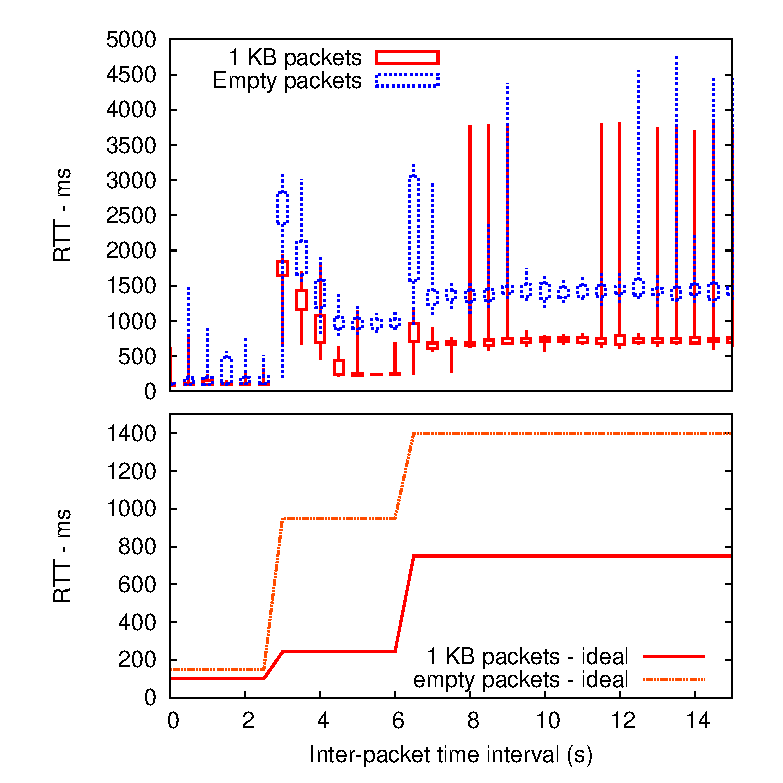
\includegraphics[width=0.45\textwidth]{figs/test_rrc_bad.eps}
\end{center}
\ncaption{Top graph: 22 measurements of RTTs as a function of time between packets. Ideally, we would expect it to appear like the lower, ideal graph, with no transmissions delays.}
\label{fig:rtt_raw_data_22}
\vspace{2ex}
\end{figure}

In developing these algorithms, we made use of three test devices, covering two models of phone and two carriers. \TReport{We examined T-Mobile and AT\&T, using one Samsung Galaxy SIII for each carrier as well as an HTC one on T-Mobile.}
We used QxDM to verify the ground truth for network timings for two of these devices, as well as to verify the presence of the anomalous FACH\_{}TRANSITION behavior and to determine the impact of RLC-layer transient states. We also validated our findings with a power monitor, as in previous work~\cite{3g_rrc, 4g_rrc}. Finally, in a controlled study with various devices on a single carrier\TReport{, T-Mobile,} using known RRC state machines (as described in \S\ref{sec:clientresults}) we verified that our inference algorithm is effective, including in higher-noise conditions. We also determined how much data is insufficient for the algorithm to work.  We compare our inferred timers with the QxDM-derived ground truth in \S\ref{sec:qxdm.analysis}.

We start by describing the client design below.

%Similar to the inference technique described in previous work~\cite{3g_rrc}, the core idea is to send a UDP packet that ensures the device starts in DCH state, then wait successively longer intervals before sending an additional UDP packet - either one large enough to always trigger a promotion to DCH, or a small one that can potentially be sent while remaining in FACH.  An echo server sends a packet back immediately so that the round-trip time of these two  packet types can be measured to deduce whether the device is in DCH, FACH or PCH.  A set of heuristics have been defined to identify which is which.

% TODO list heuristics before and after?

%First, as we have shown in our motivating example, it is not always entirely accurate to say that data falls into three clean, discrete and easy to identify states.  Even in IDLE or PCH, there can be significant differences between large and small packet RTTs (which makes our FACH heuristic a problem).  Furthermore, state transitions appear to often cause significant changes in RTTs - a number of ``pseudo-states" can appear, which can confuse a naive inference implementation. Just as importantly, it is this device- and carrier-specific anomalous behavior that we are trying to measure.

%Furthermore, this approach is tied to a specific network technology.  We do not want to have different algorithms for 3G, 2G and LTE if possible --- a general solution is much cleaner.  A generic state inference algorithm that can capture all of this anomalous behavior would be ideal.

%Additionally, we found that, while data that has been collected in the past is relatively noise-free, in practice the data collected can be very noisy, especially with weaker signal strengths.  This becomes particularly significant when trying to distinguish anomalous behavior during state transitions.  Is there a spike in RTTs due to delays on the network, or due to RTT-related delays?  If we have data from a small number of tests, this might not be obvious.  Even with many samples, it is valuable to be able to easily and efficiently determine the underlying RRC state patterns.

%Finally, in LTE specifically, many of the timers involved are very short, and very difficult to infer accurately due to the high level of noise in RTT measurements.  We investigate the feasibility of inferring these shorter timers, and show that, with the exception of those on the order of milliseconds, it is possible to infer these timers using packets to probe actively.  However, as there is significantly more overhead in detecting these fine-grained timers than in detecting timers on the order of seconds, we do not include this inference technique in our broader survey of RRC states.

\subsection{RRC Inference Client Design}
\begin{algorithm}[t!]\small
\begin{algorithmic}
\STATE {\textit{\textbf{Function} ClientDemotionTest():}}
\FOR{$n=0$ to $30$ inclusive} 
\FOR{$i=0$ to $9$} 
\STATE Send \emph{max} bytes, server echoes \emph{min} bytes.
\STATE Sleep $500n$ ms.
\STATE Send ten \emph{max} bytes, server echoes \emph{min} byte for each.
\STATE Record average RTT and packets lost (7s timeout).
\STATE Sleep $500n$ ms.
\STATE Send ten \emph{min} bytes, server echoes \emph{min} byte for each.
\STATE Record average RTT and packets lost (7s timeout).
\IF {No other traffic sent}
\STATE{record RTTs and losses}
\STATE{break from inner loop}
\ENDIF
\ENDFOR
\ENDFOR
\end{algorithmic}
\caption{Client-side data collection}
\label{alg:client_collection}
%\vspace{-0.5em}
\end{algorithm}

%\begin{TReport}
%\begin{algorithm}[t!]
%\begin{algorithmic}
%\STATE {\textit{\textbf{Function} FindDemotionModel:}}
%\FORALL{test runs from client}
%\STATE smoothData(smallPackets)
%\STATE smoothData(largePackets)
%\ENDFOR
%\FORALL{inter-packet time intervals}
%\STATE remove outliers and average across tests
%\ENDFOR
%\IF {Less than 10 complete tests}
%\STATE smooth all data again
%\ENDIF
%\STATE smallModel $\leftarrow$ Divide smallPackets into segments with similar RTTs
%\STATE largeModel $\leftarrow$ Divide largePackets into segments with similar RTTs
%\IF {time ranges of smallModel and largeModel inconsistent}
%\IF {differ by one data point}
%\STATE Pick segment range with smallest average error on measured data
%\STATE Re-calculate segment average values for the other model
%\ELSE
%\STATE Split larger mis-matched segment to align with other model
%\STATE Re-calculate segment average values for the  model
%\ENDIF
%\ENDIF
%\end{algorithmic}
%\ncaption{Server-side post-processing}
%\label{alg:client_collection}
%\end{algorithm}
%
%\begin{algorithm}[t!]
%\begin{algorithmic}
%\STATE {\textit{\textbf{Function} smoothData(data):}}
%\FOR{$i$ from $1$ to length(data) $-1$}
%\STATE d $\leftarrow \lvert data\lbrack i + 1 \rbrack - data\lbrack i - 1 \rbrack \lvert$
%\IF {$d < \frac{data\lbrack i - 1 \rbrack}{4}$}
%\STATE $newData\lbrack i \rbrack \leftarrow \frac{data\lbrack i + 1 \rbrack + data\lbrack i - 1 \rbrack}{2}$
%\ELSE 
%\STATE $newData\lbrack i \rbrack \leftarrow data\lbrack i \rbrack$
%\ENDIF
%\ENDFOR
%\RETURN newData
%\end{algorithmic}
%\ncaption{data smoothing algorithm used in server-side post-processing}
%\label{alg:client_collection}
%\end{algorithm}
%
%\begin{algorithm}
%\begin{algorithmic}
%\STATE {\textit{\textbf{Function} createPreliminaryModel(data, nCompleteTests):}}
%\STATE currentSegment $\leftarrow \lbrack \rbrack$
%\IF {more than 10 complete tests}
%\STATE $r1 \leftarrow 0.25$; $r2 \leftarrow 0.5$; $r3 \leftarrow 0.75$
%\STATE $in_spike \leftarrow 1$; $min_normal \leftarrow 2$
%\ELSE
%\STATE $r1 \leftarrow 0.5$; $r2 \leftarrow 0.75$; $r3 \leftarrow 1$
%\STATE $min_{spike} \leftarrow 2$; $min_normal \leftarrow 3$
%\ENDIF
%\FOR{$i$ from $1$ to length(data)}
%\IF {currentSegment is empty}
%\STATE {Add $data\lbrack i \rbrack$}
%\ELSE
%\STATE avg $\leftarrow$ average over data in currentSegment
%\STATE $d \leftarrow \lvert avg - data\lbrack i \rbrack\lvert$
%\IF {$d < 200$ \AND $\frac{diff}{avg} > r2$ \AND items in currentSegment $> min_normal$ }
%\STATE Save start, end and average value of segment, and start new segment 
%\ELSIF {$200 < d < 1700 $ \AND $\frac{diff}{avg} > r1$ \AND items in currentSegment $>min_normal$}
%\STATE Save start, end and average value of segment, and start new segment 
%\ELSIF {$d > 200$ \AND $\frac{diff}{avg} > r3$ \AND items in currentSegment $>min_{spike}$}
%\STATE 
%\ELSE 
%\STATE Add $data\lbrack i \rbrack$ to currentSegment
%\ENDIF
%\ENDIF
%\ENDFOR 
%\STATE Return all segments generated 
%\end{algorithmic}
%\ncaption{Create Preliminary Model for RRC Inference; differ by test size to conservatively ignore RTT spikes on small data sets.}
%\label{alg:client_collection}
%\end{algorithm}
%\end{TReport}

Data is collected client-side, and a server script generates an RRC state model for each device based on all data collected to date.  This allows for a relatively lightweight client application as well as allowing the RRC state model to be improved over time. We use the example of 3G  UMTS below, but this approach applies to LTE and \textit{Enhanced Data rates for GSM Evolution} (EDGE) as well.

The client design is based on previous work~\cite{3g_rrc}, although substantial changes were needed to enable a real-world deployment and for anomalous transition states to be detected. Algorithm~\ref{alg:client_collection} summarizes the client design. In previous work, DCH is induced by sending a 1 KB UDP packet, then another UDP packet after a specified period of time, which is either empty or 1 KB, so that state transitions dependent on the quantity of data sent could be identified. The server echoes back an empty packet so the RTT can be calculated --- an empty packet is chosen to minimize the effect of queueing on the return path. Differences in RTT allow the RRC state for each inter-packet timing to be determined, and thus the RRC state timers.  

In previous work, a straightforward classification approach was used.  If the \textit{round-trip time} (RTT) is small, it is in DCH; if there is a long delay it is in PCH, as the delay implies a promotion has occurred.  If the delay of the small packet is substantially smaller than the large one, it is likely in FACH, where a promotion to DCH occurs only when the data in the buffer exceeds a certain size.  Similar packet timing patterns occur for other technologies; for LTE, RRC\_{}CONNECTED follows a similar pattern to DCH, and RRC\_{}IDLE is similar to PCH. Our classification approach is similar, but allows us to detect unexpected phenomena --- for example, due to transition delays we can no longer safely assume that DCH is associated with the longest RTT.


There are several modifications that need to be made to this algorithm.  Network characteristics and RRC implementations have changed since the previous study was performed in 2010~\cite{3g_rrc}, so some assumptions made then do not hold. In particular, anomalous transition behavior has become common and we wish to study this phenomenon.  Changes also need to be made so that the tool can be used as part of a public deployment, as there were numerous practical limitations to the tool from previous work. 

First, we modify how we collect data to ensure that timers are accurately inferred. Inter-packet timings are increased at half-second intervals and only measure from 0 to 15 seconds, instead of increasing by second intervals over 30 seconds.  Since the previous study, timers have become shorter and half-seconds now make a significant difference.  As well, for efficiency we measure the timings for large and small packets together. Each individual subtest for a specific inter-packet timing $n$ is performed as follows: a 1 KB packet is sent to induce DCH, then there is a $n$-second delay, then 1 KB test packets are sent, then there is another $n$-second delay, then  empty test packets are sent.  We send 10 packets for each test to count losses, as well as record the signal strength values.  This data is sent to the server for processing.

We collect data for all inter-packet timings, as opposed to taking a binary-search approach, because RRC state is often not apparent from a single sample.  For timers of 1100 and 1500, for example, the device appears to be in PCH, but it might instead be experiencing high network delays or be in an anomalous transition state.
 
Changes are also made to make the algorithm suitable for a public deployment in an Android application. We need to ensure no interfering network traffic is sent by the device that might unexpectedly alter the RRC state.  We also do not want users to need to do anything beyond installing the application. We make use of global packet count information in  /proc/net/dev to verify that no interfering traffic has been sent for our tests.  After 15 failed tries to measure an inter-packet interval, we record the test was unsuccessful, as the device may be under heavy use at the time.

In the best case, where every try succeeds, the test will take just under 8 minutes.  In practice, in controlled experiments it usually took twenty to thirty minutes.  

We also record the effects of RRC state on higher-level protocols.  We record tests in the middle of each inferred RRC state. We record the impact of RRC state on DNS lookups, TCP handshakes, and HTTP connections.

This methodology is only suitable for timers at the granularity of half-seconds.  For 3G this is not a problem, as timers are generally on the order of seconds.  For LTE, the timer for the transition between RRC\_CONNECTED and RRC\_IDLE is similarly on the order of seconds. However,  some of the timers for the states within RRC\_CONNECTED can be as small as 20 ms, and even the RRC\_IDLE cycle length requires measurements several times a second to detect~\cite{4g_rrc}.  

We have explored various approaches to measuring these timers.  There are three main challenges: there is a great deal of noise in the network; the Android framework introduces additional unexpected delays; and measuring these short timers increases the amount of traffic that needs to be sent by several orders of magnitude. We were able to substantially increase the accuracy of our RTT measurements by collecting tcpdump~\cite{tcpdump} traces, but this was insufficient. We found that even after sending packets continuously from one device for days, it was not possible to reliably and accurately infer these small packet timers.  



%This introduces a number of challenges.

%First, measuring at finer granularities significantly increases the number of measurements clients make and the time taken to complete a test by a factor of 25.  As tests in high-traffic conditions can take as long as an hour, this is evidently not ideal.  Furthermore, measuring inter-packet intervals and round-trip times at 20 ms granularities is hard for several technical reasons as well.  

%First of all, there is a significant amount of jitter on cellular networks, and a great deal of data needs to be collected in order to accurately measure these values. This effect can be seen in Figure~\ref{fig:LTE_development} --- compare the noisiness of data to that in Figure~\ref{fig:rtt_raw_data_22}.  For both our fine-grained and coarse-grained inference tasks, four to five tests are needed to consistently remove outliers.

% TODO give some concrete values + graphs based on LTE tests here. A graph of an LTE test vs one of a coarse-grained 3G test is a clear indication of the problem.

%Another problem is that delays are introduced due to scheduling and overhead when implemented at the Android Framework level (i.e. in Dalvik).  A native code implementation would give us much more accurate timer and RTT values; we leave this to future work.  We have instead on several devices prototyped a packet inference system using tcpdump traces~\cite{tcpdump} to measure accurate inter-packet timings.  Using this, we were able to eliminate much of the jitter that was preventing us from taking accurate measurements and were able to infer the timer to transition from Short DRX to Long DRX as well as the cycle period of RRC\_IDLE, but were not able to infer the shorter timers in this way.  An example of the data collected for which we were able to infer these states can be seen in Figure~\ref{fig:LTE_development}.

We also investigated the possibility of performing all measurements passively.  By monitoring packet counters in /proc/net/dev/, it is possible to see when packets are being sent and received by existing applications on the device, thus eliminating the cost in terms of data overhead.  We monitored the packets sent and received on an actively used device for a week, and found that the range of inter-packet timing intervals was not sufficiently varied to reach any useful conclusions during that time.  As continuously monitoring background traffic in this manner can have a significant impact on battery life, this does not appear to be a feasible solution.

UMTS demotion patterns are detected in the same manner as in previous work~\cite{3g_rrc}.  We do not currently infer the buffer sizes that need to be exceeded to trigger a transition from FACH to DCH, but this could be done using a binary-search approach, by sending packets of various sizes in order to determine at what point the RTT changes substantially.

%Question: do we have something to cite on this problem?


\subsection{RRC Inference Server Design}

\begin{figure}[t!]
\begin{center}
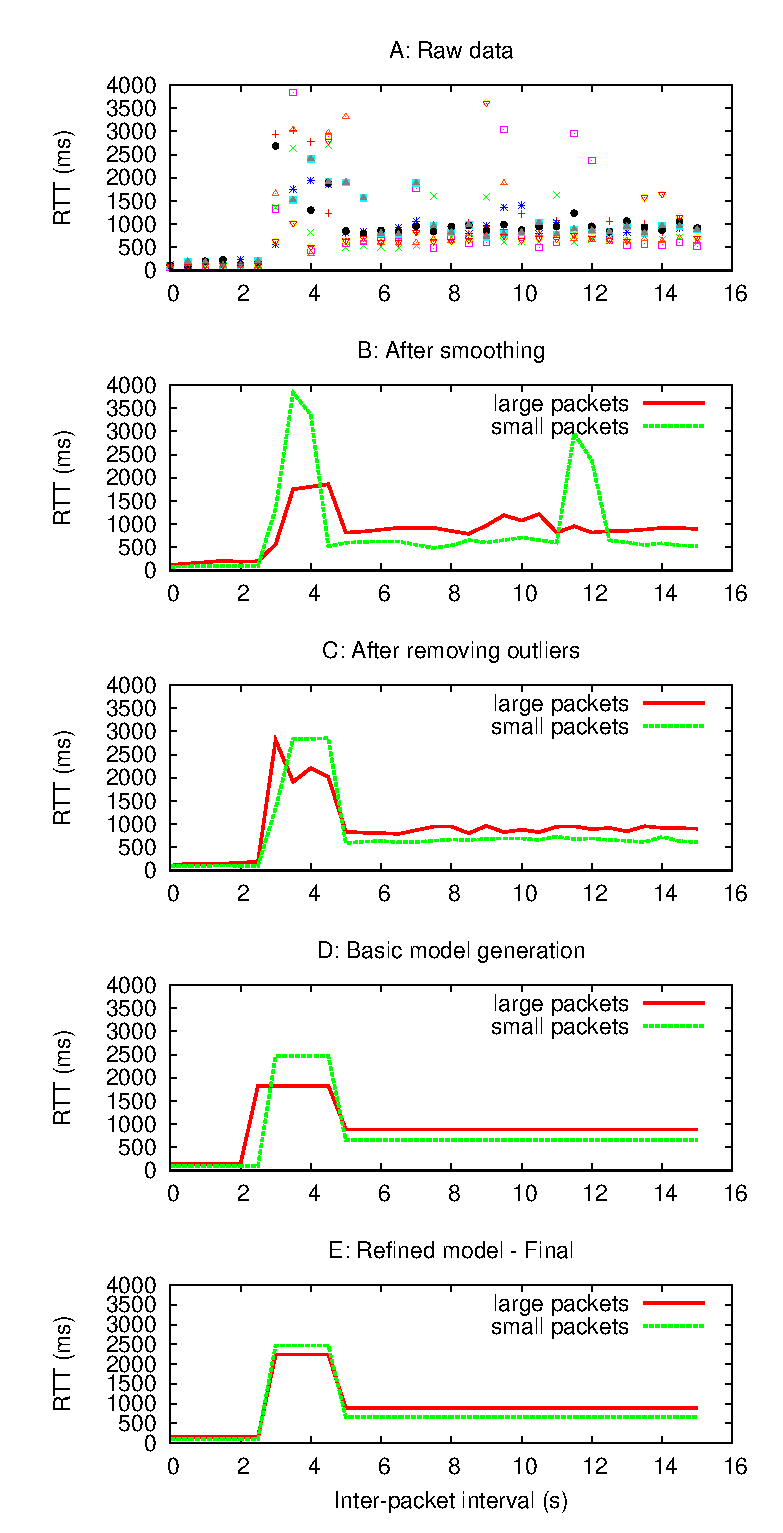
\includegraphics[width=0.5\textwidth]{figs/model_generation.eps}
\end{center}
\ncaption{Steps in extracting RRC model and unexpected behavior trends from raw data.  Note that the raw data follows a non-ideal pattern. Step B: modified running average function that preserves state transitions applied to one test only.  Step C: all tests averaged without outliers removed. Step E: DCH and PCH state extracted; in between them is RRC\_{}TRANSITION rather than FACH --- the anomalous transition period occurs throughout the entire FACH state.}
\label{fig:model_development}
\end{figure}

Aside from storing our results, the server's main role is generating the RRC state models.  Upon uploading a new set of data, a new model is generated for that device ID. To deal with the higher level of noise in our data as well as to be able to analyze all network types and detect unexpected behavior, it was necessary to take an entirely different approach to the server-side analysis from what was done in previous work~\cite{3g_rrc}.

In the ideal case, the data would closely fit the ideal RRC state behavior.  In practice, even in the best case it looks more like Figure~\ref{fig:rtt_raw_data_22}, where there are spikes in latency around RRC transmissions, as well as noise in high-latency RRC states.  There may be far fewer measurements for a device, and the data collected is often noisier. Furthermore, we would like to observe when devices behave in unexpected ways. 

 To create a reasonable RRC model under adverse conditions, we first remove noise from the data, and then divide into timer ranges where RRTs are similar.  Finally, we label the states detected where possible.  We treat 1 KB packets differently from empty packets.  The FACH state is characterized by these packets having very different values and therefore we wish to ensure these differences are preserved.

Filtering noise is not always straightforward, as interesting phenomena such as high round-trip times surrounding state transitions can look like intermittent delays, and vice-versa.  We experimented with several noise filtering approaches on four devices with different manufacturers and carriers to develop our filtering approach before verifying with a larger number of devices.  Taking the average value of all tests was not effective, as these values are often skewed by high amounts of noise.  Taking median values is more effective, but it is also sensitive to periodic noise spikes, especially for small numbers of tests. We also tried taking the minimum value of a set of tests, the intuition being that the network is likely to add delays but not subtract them, but this also resulted in noisy data.

There were two approaches that did work well, however, which are complementary. The first is to remove outliers. If there are three tests, with round-trip times 132, 145 and 370, then most likely the third one is due to intermittent delay.  We disregard all values that are more than half a standard deviation from the mean, or one standard deviation when less than ten tests were performed, then average the remaining values.  This significantly reduces noise in our data in most cases. However, for very noisy data and few tests this still often leaves noise spikes.  If there are three tests, and two coincidentally happen to have latency spikes at the same time, then this spike will not be filtered out.

A modified running average function applied to the data is also effective.  We call this our ``smoothing" function, which is applied to individual tests. For every data point, we first consider the difference between the points on either side of that point.   If this difference is more than a quarter of the data point in question, we leave it as is.  Otherwise, the data point is updated to be the average of the points before and after it. This has two results: first, we filter latency spikes, and second, we do not smooth large jumps in the data which are characteristic of state transitions.

These two approaches complement each other.  Smoothing works well when the probability of a latency spike for each data point is independent, but works poorly where there are consistent RTT delays for several consecutive tests.  Outlier removal works well when a specific test has latency spikes that other tests do not, and especially when a specific test has much longer RTTs than the others. It does not work well for very high levels of random noise.  

After experimenting with various orderings for these two approaches on a number of devices, we found that smoothing each test individually before removing outliers between the tests performs best.  If we remove outliers first, then for noisy data we may inadvertently filter out the correct, low-noise values.  We then smooth the data again at the end to make the data to process cleaner.  The results of these steps can be seen in Figure~\ref{fig:model_development}, parts B and C. B shows the results of smoothing a single test only.

After these pre-processing steps, we create the model. At first, we continue to treat small and large packets separately.  Starting with the smallest interpacket interval, we divide the data into segments with approximately constant round-trip times. The results of this can be seen in Figure~\ref{fig:model_development}, part D.

Then, we compare the two models generated --- that for the large packets, and that for the small packets.  Although the average RTT for the two models differs, the beginning and end of each segment should be the same for both. There are two cases where the boundaries of segments may differ after model generation that need to be corrected.   First, with low amounts of data, it sometimes happens that the beginning and end of a segment for each model is off by half a second.  An example can be seen in Figure~\ref{fig:model_development}, part D. In this case, we find which segment division will result in the smallest average error and apply that to both models.  Second, there are some states where behavior for one packet size or the other does not change.  In particular, in the FACH state it is possible that the RTT for small packets is very close to that in DCH state.  In this case, we split the larger segment.  

Finally, we label the states. We do not use the same assumptions in doing so as in previous work as we find these do not always apply to our data. In particular, we do not assume that in PCH the 1KB packets and empty packets have very similar delays, as we find that this is frequently not the case.  Instead, we determine states based on the relative average RTTs of each segment.  For example, FACH (by definition) has latencies for empty packets close to those in DCH, whereas PCH does not. We also account for the fact that we expect to see states appear in a particular order as we increase inter-packet timings. For example, a carrier implementing the UMTS specification will never demote to FACH after demoting to PCH with no packets being sent.  

This step was first developed and validated on a small number of devices whose behavior was verified using QxDM. It was also validated using an internal deployment on a carrier with known RRC state machine timers.


We look for the following states: high-power (DCH-like), low-power (PCH-like), and FACH-like.  We also look for latency spikes transitioning between these states, like that seen in Figure~\ref{fig:model_development}.  Anything that does not fit one of these patterns we label as ``Anomalous" and flag for manual investigation.  We err on the side of flagging models as anomalous to ensure that all other RRC states are accurate. We describe these results in \S\ref{sec:clientresults}.

%\subsection{LTE Short Timers}
%
%\begin{figure}[t!]
%\begin{center}
%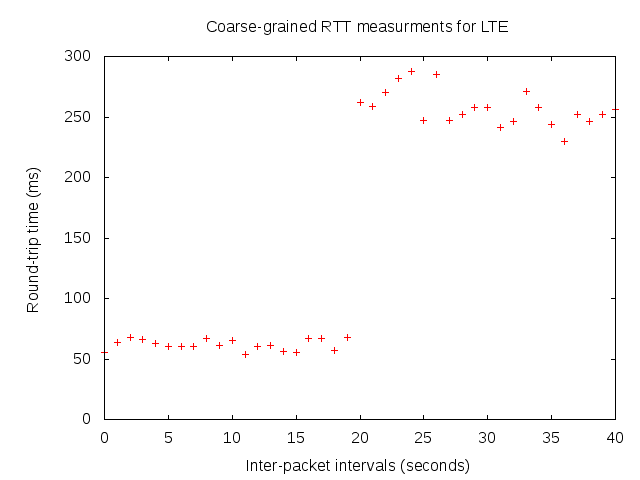
\includegraphics[width=0.45\textwidth]{figs/lte_naive.png}
%\end{center}
%\ncaption{Example data collected for LTE using coarse-grained measurement approach}
%\label{fig:LTE_raw}
%\end{figure}
%
%\begin{figure}[t!]
%\begin{center}
%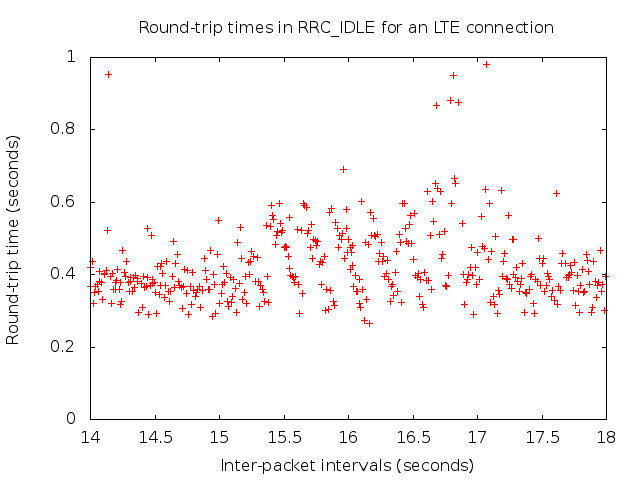
\includegraphics[width=0.45\textwidth]{figs/lte_idle.png}
%\end{center}
%\ncaption{Example data collected for short LTE timers in RRC\_IDLE, focusing on lowest-noise region of test}
%\label{fig:LTE_detailed}
%\end{figure}
%
%
%\begin{figure}[t!]
%\begin{center}
%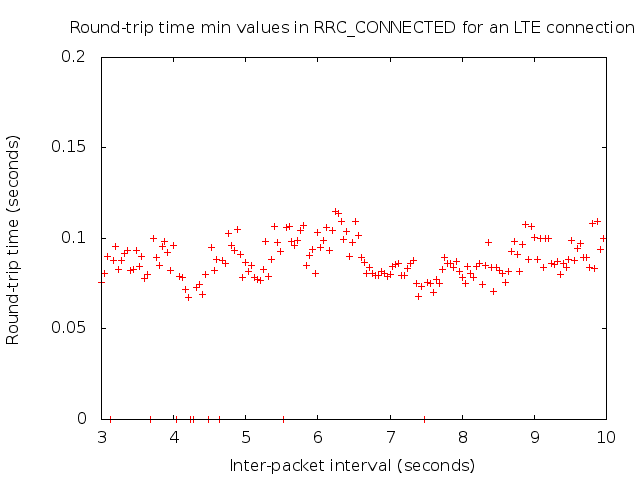
\includegraphics[width=0.45\textwidth]{figs/lte_connected.png}
%\end{center}
%\ncaption{Example data collected for short LTE timers in , focused on }
%\label{fig:LTE_connected}
%\end{figure}
%
%
%This methodology is only suitable for timers at the granularity of half-seconds, evidently.  For 3G this is not a problem, as timers are generally on the order of seconds.  For LTE, the timer for the transition between RRC\_CONNECTED and RRC\_IDLE isisimilarly on the order of seconds. However, as was shown in previous work~\cite{4g_rrc}, some of the timers for the states within RRC\_CONNECTED can be as small as 20 ms, and even the RRC\_IDLE cycle length requires measurements several times a second to detect.  Furthermore, as boundaries for these ``sub-states" are not derived by detecting step functions but rather sawtooth shapes, to accurately detect these timers measurements need to be taken at time intervals several times shorter than the timers that are being inferred.
%
%This introduces a number of challenges, and requires modifications to client-side and server-side code.  We were able to infer timers on the order of 100ms, but probably any on the order of 10ms would not be feasible.
%
%Evidently, it is necessary to send data at much higher frequencies.  Instead of having inter-packet intervals increasing with increments of half-seconds, we have intervals increasing with increments of ten milliseconds.  This does, however, increase the number of tests that need to be done by a factor of fifty, and the length of time needed to complete a single test from tens of minutes to tens of hours.  As a result, we have performed these tests only on devices specifically meant for that purpose.
%
%Additonally, there is the problem that there is a significant amount of jitter on cellular networks, and a great deal of data needs to be collected in order to accurately measure these values. This effect can be seen in Figure~\ref{fig:LTE_raw} --- compare the noisiness of data to that in Figure~\ref{fig:rtt_raw_data_22}.  
%
%A large source of this problem is that delays are introduced due to scheduling and overhead when implemented at the Android Framework level (i.e. in Dalvik).   Both the values collected and the precise length for which the timers run are not accurate to the millisecond. We found that timer values, in particular, are incorrect on average by 3.3 ms, with a standard deviation of 2.8 ms, which could have a substantial impact on timers on the order of 10ms. It is possible to implement our application in C and have it run natively, using the Android NDK.  As a proof-of-concept, we have collected measurements using tcpdump~\cite{tcmpdump} instead, and extract inter-packet timings and RTT values directly. Using this, we were able to eliminate much of the jitter that was preventing us from taking accurate measurements.
%
%Even so, the data we receive can often be quite noisy.  For the idle period in RRC\_IDLE, it suffices to simply perform enough tests that the characteristic sawtooth pattern becomes evident (see Figure~\ref{fig:LTE_detailed}).  In our controlled experiment, one such set of data appeared in our first test performed.  However, for the timers on the order of tens of milliseconds, this is still insufficient.  To recover these, we perform several complete tests, bin inter-packet timings into 10-ms intervals, and take the minimum value of all data points.  This pre-processing step is sufficient to extract these smaller timers, as can be seen in Figure~\ref{fig:LTE_connected}.
%
%Due to the high energy and data cost of these tests, we currently limit them to controlled experiments, and as such in \S~\ref{sec:clientresults} where we perform a large-scale evaluation of global RRC state machines, we focus only on the coarse-grained timers for our LTE measurements.  Crowd-sourcing these timers seems impractical, as the battery cost would probably mean this measurement would not be worthwhile for the average user, but it is certainly possible for an interested expert to infer most LTE timers in this manner. 
%
%\mycomment{Measurements taken with power monitor to verify may suggest these values are not accurate. May change writing to reflect that.}
%
%RRC inference can help us detect new sources of delays, packet loss, and other performance problems, but it does not allow us to understand \emph{why} the unexpected phenomena that we detect occur.  For that, we need to examine lower-level behavior directly.  In the next section, we discuss how we approach this problem and address the issues in understanding RLC-level behavior.
%
%In short, we have significantly improved RRC state inference. We have shown that it is possible to collect network data for RRC inference on arbitrary devices using an application running in the background, without requiring any special expertise, device modifications, or any similar burdens on the users.  We have also found that it is possible to infer very shorty timers associated with LTE states which could not previously be measured.
